% Options for packages loaded elsewhere
\PassOptionsToPackage{unicode}{hyperref}
\PassOptionsToPackage{hyphens}{url}
%
\documentclass[
  a4paper,
]{scrbook}

\usepackage{amsmath,amssymb}
\usepackage{lmodern}
\usepackage{iftex}
\ifPDFTeX
  \usepackage[T1]{fontenc}
  \usepackage[utf8]{inputenc}
  \usepackage{textcomp} % provide euro and other symbols
\else % if luatex or xetex
  \usepackage{unicode-math}
  \defaultfontfeatures{Scale=MatchLowercase}
  \defaultfontfeatures[\rmfamily]{Ligatures=TeX,Scale=1}
\fi
% Use upquote if available, for straight quotes in verbatim environments
\IfFileExists{upquote.sty}{\usepackage{upquote}}{}
\IfFileExists{microtype.sty}{% use microtype if available
  \usepackage[]{microtype}
  \UseMicrotypeSet[protrusion]{basicmath} % disable protrusion for tt fonts
}{}
\makeatletter
\@ifundefined{KOMAClassName}{% if non-KOMA class
  \IfFileExists{parskip.sty}{%
    \usepackage{parskip}
  }{% else
    \setlength{\parindent}{0pt}
    \setlength{\parskip}{6pt plus 2pt minus 1pt}}
}{% if KOMA class
  \KOMAoptions{parskip=half}}
\makeatother
\usepackage{xcolor}
\setlength{\emergencystretch}{3em} % prevent overfull lines
\setcounter{secnumdepth}{5}
% Make \paragraph and \subparagraph free-standing
\ifx\paragraph\undefined\else
  \let\oldparagraph\paragraph
  \renewcommand{\paragraph}[1]{\oldparagraph{#1}\mbox{}}
\fi
\ifx\subparagraph\undefined\else
  \let\oldsubparagraph\subparagraph
  \renewcommand{\subparagraph}[1]{\oldsubparagraph{#1}\mbox{}}
\fi


\providecommand{\tightlist}{%
  \setlength{\itemsep}{0pt}\setlength{\parskip}{0pt}}\usepackage{longtable,booktabs,array}
\usepackage{calc} % for calculating minipage widths
% Correct order of tables after \paragraph or \subparagraph
\usepackage{etoolbox}
\makeatletter
\patchcmd\longtable{\par}{\if@noskipsec\mbox{}\fi\par}{}{}
\makeatother
% Allow footnotes in longtable head/foot
\IfFileExists{footnotehyper.sty}{\usepackage{footnotehyper}}{\usepackage{footnote}}
\makesavenoteenv{longtable}
\usepackage{graphicx}
\makeatletter
\def\maxwidth{\ifdim\Gin@nat@width>\linewidth\linewidth\else\Gin@nat@width\fi}
\def\maxheight{\ifdim\Gin@nat@height>\textheight\textheight\else\Gin@nat@height\fi}
\makeatother
% Scale images if necessary, so that they will not overflow the page
% margins by default, and it is still possible to overwrite the defaults
% using explicit options in \includegraphics[width, height, ...]{}
\setkeys{Gin}{width=\maxwidth,height=\maxheight,keepaspectratio}
% Set default figure placement to htbp
\makeatletter
\def\fps@figure{htbp}
\makeatother

\usepackage{cancel}
\makeatletter
\@ifpackageloaded{tcolorbox}{}{\usepackage[many]{tcolorbox}}
\@ifpackageloaded{fontawesome5}{}{\usepackage{fontawesome5}}
\definecolor{quarto-callout-color}{HTML}{909090}
\definecolor{quarto-callout-note-color}{HTML}{0758E5}
\definecolor{quarto-callout-important-color}{HTML}{CC1914}
\definecolor{quarto-callout-warning-color}{HTML}{EB9113}
\definecolor{quarto-callout-tip-color}{HTML}{00A047}
\definecolor{quarto-callout-caution-color}{HTML}{FC5300}
\definecolor{quarto-callout-color-frame}{HTML}{acacac}
\definecolor{quarto-callout-note-color-frame}{HTML}{4582ec}
\definecolor{quarto-callout-important-color-frame}{HTML}{d9534f}
\definecolor{quarto-callout-warning-color-frame}{HTML}{f0ad4e}
\definecolor{quarto-callout-tip-color-frame}{HTML}{02b875}
\definecolor{quarto-callout-caution-color-frame}{HTML}{fd7e14}
\makeatother
\makeatletter
\makeatother
\makeatletter
\@ifpackageloaded{bookmark}{}{\usepackage{bookmark}}
\makeatother
\makeatletter
\@ifpackageloaded{caption}{}{\usepackage{caption}}
\AtBeginDocument{%
\ifdefined\contentsname
  \renewcommand*\contentsname{Table of contents}
\else
  \newcommand\contentsname{Table of contents}
\fi
\ifdefined\listfigurename
  \renewcommand*\listfigurename{List of Figures}
\else
  \newcommand\listfigurename{List of Figures}
\fi
\ifdefined\listtablename
  \renewcommand*\listtablename{List of Tables}
\else
  \newcommand\listtablename{List of Tables}
\fi
\ifdefined\figurename
  \renewcommand*\figurename{Figure}
\else
  \newcommand\figurename{Figure}
\fi
\ifdefined\tablename
  \renewcommand*\tablename{Table}
\else
  \newcommand\tablename{Table}
\fi
}
\@ifpackageloaded{float}{}{\usepackage{float}}
\floatstyle{ruled}
\@ifundefined{c@chapter}{\newfloat{codelisting}{h}{lop}}{\newfloat{codelisting}{h}{lop}[chapter]}
\floatname{codelisting}{Listing}
\newcommand*\listoflistings{\listof{codelisting}{List of Listings}}
\makeatother
\makeatletter
\@ifpackageloaded{caption}{}{\usepackage{caption}}
\@ifpackageloaded{subcaption}{}{\usepackage{subcaption}}
\makeatother
\makeatletter
\@ifpackageloaded{tcolorbox}{}{\usepackage[many]{tcolorbox}}
\makeatother
\makeatletter
\@ifundefined{shadecolor}{\definecolor{shadecolor}{rgb}{.97, .97, .97}}
\makeatother
\makeatletter
\makeatother
\ifLuaTeX
  \usepackage{selnolig}  % disable illegal ligatures
\fi
\IfFileExists{bookmark.sty}{\usepackage{bookmark}}{\usepackage{hyperref}}
\IfFileExists{xurl.sty}{\usepackage{xurl}}{} % add URL line breaks if available
\urlstyle{same} % disable monospaced font for URLs
\hypersetup{
  pdftitle={zero-to-hero},
  pdfauthor={Ed Southwood},
  hidelinks,
  pdfcreator={LaTeX via pandoc}}

\title{zero-to-hero}
\author{Ed Southwood}
\date{09/09/2022}

\begin{document}
\frontmatter
\maketitle
\ifdefined\Shaded\renewenvironment{Shaded}{\begin{tcolorbox}[sharp corners, boxrule=0pt, borderline west={3pt}{0pt}{shadecolor}, breakable, frame hidden, enhanced, interior hidden]}{\end{tcolorbox}}\fi

\renewcommand*\contentsname{Table of contents}
{
\setcounter{tocdepth}{2}
\tableofcontents
}
\mainmatter
\bookmarksetup{startatroot}

\hypertarget{welcome}{%
\chapter*{Welcome}\label{welcome}}
\addcontentsline{toc}{chapter}{Welcome}

This course is designed to refresh your knowledge of maths to get you
ready to use calculus in your course. There is no right or wrong way to
use it. Each section includes written notes, a video (with the same
content as the notes) and practice questions. It's chunked into
bitesized sections to allow you make progress in 10 min windows. You may
like to try the questions first and then just go back to the notes if
you get stuck. Feel free to start anywhere you like.

This is a work in progress, the videos are appearing and things may
change! If you find a mistake please email edrs20@bath.ac.uk and good
luck!

\bookmarksetup{startatroot}

\hypertarget{negative-numbers}{%
\chapter{Negative numbers}\label{negative-numbers}}

On a number line negative numbers are typically written to the left of
zero and have values smaller than zero. Negative numbers are tricky.
Often when an error creeps into a calculation it's due to a misplaced
minus sign, they are a source of problems for everyone - don't worry if
they seem tricky, they have only relatively recently lost their
mysteriousness. The evidence of humans counting dates from \(35,000\)BCE
yet as recently as \(1758\) British mathematician Francis Maseres said
that negative numbers\ldots{}

\emph{``\ldots{} darken the very whole doctrines of the equations and
make dark of the things which are in their nature excessively obvious
and simple''.}

\hypertarget{multiplication-and-division}{%
\section{Multiplication and
Division}\label{multiplication-and-division}}

When multiplying and dividing using negative numbers the answer will be
the same as the equivalent calculation with positive numbers only, but,
you may have to change the sign - to either positive or negative. The
rules for deciding if the answer is positive or negative are below:

\begin{tcolorbox}[enhanced jigsaw, opacityback=0, left=2mm, toptitle=1mm, title=\textcolor{quarto-callout-note-color}{\faInfo}\hspace{0.5em}{Note}, breakable, colbacktitle=quarto-callout-note-color!10!white, opacitybacktitle=0.6, bottomtitle=1mm, arc=.35mm, colback=white, leftrule=.75mm, bottomrule=.15mm, colframe=quarto-callout-note-color-frame, rightrule=.15mm, titlerule=0mm, toprule=.15mm, coltitle=black]

\begin{itemize}
\tightlist
\item
  positive \(\times\) positive \(=\) positive
\item
  negative \(\times\) positive \(=\) negative
\item
  positive \(\times\) negative \(=\) negative
\item
  negative \(\times\) negative \(=\) positive
\end{itemize}

\end{tcolorbox}

Notice that the order is not important. Here are some examples:

\[
-2 \times 3 = -6
\]

\[
10 \times -5 = -50 
\]

\[
-4 \times -6 = 24 
\]

If you have more that two numbers to multiplying you can just count the
number of negative numbers and apply the following rule:

\begin{tcolorbox}[enhanced jigsaw, opacityback=0, left=2mm, toptitle=1mm, title=\textcolor{quarto-callout-note-color}{\faInfo}\hspace{0.5em}{Note}, breakable, colbacktitle=quarto-callout-note-color!10!white, opacitybacktitle=0.6, bottomtitle=1mm, arc=.35mm, colback=white, leftrule=.75mm, bottomrule=.15mm, colframe=quarto-callout-note-color-frame, rightrule=.15mm, titlerule=0mm, toprule=.15mm, coltitle=black]

\begin{itemize}
\tightlist
\item
  If the total number of negative numbers is \textbf{even} the answer is
  \textbf{positive}.
\item
  If the total number of negative numbers is \textbf{odd} the answer is
  \textbf{negative}.
\end{itemize}

\end{tcolorbox}

Here's a longer example:

\[
-2 \times -2 \times -2 \times -2 = 16 
\]

since there are even number of negatives in the question the answer will
be positive.

Since division and multiplication are so closely related, division works
in exactly the same way. For example:

\[
\frac{-3 \times -6}{-9} = -2 
\].

You can practice these techniques with the following questions. You can
refresh the question to change the numbers. Try them as much as you
like.

\begin{figure}

{\centering 

\href{https://numbas.mathcentre.ac.uk/question/125598/negative-numbers-multiplication-and-division/embed/}{\includegraphics{./01-negative_numbers_files/figure-pdf/unnamed-chunk-2-1.png}}

}

\end{figure}

\hypertarget{but-why}{%
\subsection{But why?!!?}\label{but-why}}

Building a physical idea of a negative number is tricky. For example
thinking of \(2 \times 3\) as two lots of 3 things is fine, but what
does \(-2 \times -3\) even mean? Hopefully but looking at the pattern
below it will be become clear that our definition of what happens with
two negative numbers is the only one that makes sense. Consider
extending the two times table into negative numbers.

\[
\begin{array}{ccccc}
3 &\times& 2& =& 6\\
2 &\times& 2& =& 4\\
1 &\times& 2& =& 2\\
0 &\times& 2& =& 0\\ 
-1 &\times& 2& =& -2\\
-2 &\times& 2& =& -4\\
-3 &\times& 2& =& -6\\ 
\end{array}
\]

Now with the negative two times table.

\[
\begin{array}{ccccc}
3 &\times& -2& =& -6\\
2 &\times& -2& =& -4\\
1 &\times& -2& =& -2\\
0 &\times& -2& =& 0\\ 
-1 &\times& -2& =& 2\\
-2 &\times& -2& =& 4\\
-3 &\times& -2& =& 6\\ 
\end{array}
\]

Our definition fits the pattern. Horrah!

\hypertarget{addition-and-subtraction}{%
\section{Addition and subtraction}\label{addition-and-subtraction}}

It helps to think about addition and subtraction of negative numbers on
a number line. We can think about positive numbers as arrows pointing
\emph{forwards}, shifts to the right from zero, and negative numbers as
arrows \emph{backwards}, shifts to the left. Add to this the idea that
addition and subtraction is then combining these arrows. When you add
two numbers you place them one after another, the end of the second
arrow on the tip of the first. With subtraction you reverse the
direction of the second arrow and then place them together just like
addition.

\includegraphics{./01-negative_numbers_files/figure-pdf/unnamed-chunk-4-1.png}

Consider the following examples:

\begin{itemize}
\tightlist
\item
  \(3 - 5 = -2\) can be thought of as: start at three then move five
  back to the left.
\item
  \(-4 + 1 = -3\), start at \(-4\) then move one to the right.
\item
  \(5 + - 2 = 3\), start at \(5\) then add on a shift of \(2\) to the
  left.
\item
  \(1 - - 3 = 4\), start at \(1\) then reverse a shift of \(3\) to the
  left (I know it seams bonkers!). The double negative cancels out to
  give a calculation equivalent to \(1 + 3 = 4\).
\end{itemize}

\begin{tcolorbox}[enhanced jigsaw, opacityback=0, left=2mm, toptitle=1mm, title=\textcolor{quarto-callout-warning-color}{\faExclamationTriangle}\hspace{0.5em}{Warning}, breakable, colbacktitle=quarto-callout-warning-color!10!white, opacitybacktitle=0.6, bottomtitle=1mm, arc=.35mm, colback=white, leftrule=.75mm, bottomrule=.15mm, colframe=quarto-callout-warning-color-frame, rightrule=.15mm, titlerule=0mm, toprule=.15mm, coltitle=black]

It's tempting to cling on to the idea that \emph{two negatives make a
positive} when it comes to addition and subtraction. But consider the
following statements, they are all correct, but imagine how easy it is
to be confused if you just apply the \emph{two negatives make a
positive} rule.

\begin{itemize}
\tightlist
\item
  \(-3 - 5 = -8\)
\item
  \(-10 - -4 = -6\)
\end{itemize}

\end{tcolorbox}

You can practice these techniques with the following questions. The
numbers change each time to try them as much as you like.

\begin{figure}

{\centering 

\href{https://numbas.mathcentre.ac.uk/question/126315/negative-numbers-addition-and-subtraction/embed/?token=1a99ce84-edc0-4467-a780-e6e9bcc6fda8}{\includegraphics{./01-negative_numbers_files/figure-pdf/unnamed-chunk-5-1.png}}

}

\end{figure}

\bookmarksetup{startatroot}

\hypertarget{algebraic-expressions}{%
\chapter{Algebraic expressions}\label{algebraic-expressions}}

Algebraic expressions are just statements about numbers. However,
letters are used as place holders for some of the numbers. There are
many reasons this is useful, it could be because we would like to
uncover the structure of something, or, because we don't know the
specific numbers to use yet.

\hypertarget{substitution}{%
\section{Substitution}\label{substitution}}

In order to evaluate an algebraic expression we have to substitute the
letters for numbers. After the numbers are written in place of the
letters we must take care to evaluate the statement in the correct
order. BIDMAS is often used to remember the order:

\begin{itemize}
\tightlist
\item
  \textbf{Brackets} Work out anything in brackets first.
\item
  \textbf{Indices} Powers are next, something like \(3^2\).
\item
  \textbf{Division and Multiplication} these two have equal priority. If
  there is a `tie' work left to right. However if you see a large
  division they have implicit brackets in them. For example
  \(\frac{2 + 10}{2 \times 3}\) should be thought of as
  \(\frac{(2 + 10)}{(2 \times 3)}\).
\item
  \textbf{Addition and Subtraction} like multiplication and division
  these are equal priority. If there is a tie work left to right.
\end{itemize}

One more thing to know before we start making substitutions is that the
multiplication symbol \(\times\) is often not used in algebraic
expressions. Letters and numbers that are next to each other are
multiplied together. For example \(3a\) means \(3 \times a\). You can
show two numbers multiplied together like this
\(2 \times 3 = (2)(3) = 6\).

Here are some examples:

If \(a=2\) and \(b=-3\) then we can evaluate \(5a + 4b\) like this:

\[
5(2) + 4(-3)
\]

When things are written next to each other this means multiplication.

\[
5\times 2 + 4 \times -3
\]

Using BIDMAS to do the multiplication first and remembering that a
positive number multiplied by a negative gives a negative number.

\[
10 +- 12 = -2
\]

Substituting \(n = 3\) and \(x = 2\) into \(5x^n\). By replacing the
letters with numbers we have:

\[
5(2)^3
\]

Remembering that when things are next to each other it means
multiplication, which gives:

\[
5 \times 2^3
\]

Following BIDMAS we must deal with the powers first. Since
\(2^3 = 2 \times 2 \times 2 = 8\) we have:

\[
5 \times 8 = 40
\]

Finally consider \(\frac{2p+q}{r}\) where \(p=6\), \(q=3\) and \(r=5\).
Replacing the letters with numbers we have:

\[
\frac{2(6)+3}{5} = \frac{2 \times 6+3}{5}
\]

Remembering that there are implicit brackets in fractions, the numerator
needs to be evaluated first.

\[
\frac{(2 \times 6+3)}{5} = \frac{(12+3)}{5}=\frac{15}{5}
\]

Now the fraction can be evaluated.

\[
\frac{15}{5} = 3
\]

You can practice these techniques with the following questions. The
numbers change each time to try them as much as you like.

\begin{figure}

{\centering 

\href{https://numbas.mathcentre.ac.uk/question/126318/algebra-substitution/embed/?token=83a5d483-0d29-43d9-9569-f3b4d04ca26e}{\includegraphics{./02-algebraic_expressions_files/figure-pdf/unnamed-chunk-1-1.png}}

}

\end{figure}

\hypertarget{simplification}{%
\section{Simplification}\label{simplification}}

Algebraic expressions are made up of terms. Similar terms can be
combined to create a simplified expression, this processes is called
\emph{collecting like terms}. For example \(2a + 3a\) can be simplified
to \(5a\) by collecting the \(a\) terms. Here's another example with a
bit more going on:

\[
5x + 7y - 3x + 3y = \overbrace{5x - 3x}^{x\text{ terms}} + \overbrace{7y + 3y}^{y\text{ terms}} = 2x + 10y
\]

Notice that the like terms were grouped first to make it easier to
simplify. Also, each term \emph{owns} the positive of negative symbol
ahead of it.

Terms can be more complex too. Although it's tempting to find something
to simplify there are no like terms in this expression:
\(3xy + 6x^2 + 2x - 5y\). Only the exact same multiples can be
simplified. For example:

\[
6x^2 + 2x - 5x^2 -8x = \overbrace{6x^2 -5x^2}^{x^2\text{ terms}} + \overbrace{2x-8x}^{x\text{ terms}}=x^2-6x
\]

Notice that the two different types of term are \(x\) and \(x^2\). Also,
I could have written \(1x^2\) but we normally don't bother with the
\(1\). It's also important to note that capitalisation matters; \(x\) is
different from \(X\).

Take care when simplifying multiples of different letters \(3xy + 5yx\)
can be simplified. This is because the order of multiplication doesn't
matter so \(3xy + 5yx = 3xy + 5xy = 8xy\). Terms are normally written in
alphabetical order with the highest powers first.

\begin{tcolorbox}[enhanced jigsaw, opacityback=0, left=2mm, toptitle=1mm, title=\textcolor{quarto-callout-note-color}{\faInfo}\hspace{0.5em}{Key point:}, breakable, colbacktitle=quarto-callout-note-color!10!white, opacitybacktitle=0.6, bottomtitle=1mm, arc=.35mm, colback=white, leftrule=.75mm, bottomrule=.15mm, colframe=quarto-callout-note-color-frame, rightrule=.15mm, titlerule=0mm, toprule=.15mm, coltitle=black]

\begin{itemize}
\tightlist
\item
  \(x \times x = x^2\)
\item
  \(x + x = 2x\)
\item
  \(x\) is different from \(X\)
\item
  \(1x\) is written as \(x\)
\end{itemize}

\end{tcolorbox}

Have a go at simplifying with these questions.

\begin{figure}

{\centering 

\href{https://numbas.mathcentre.ac.uk/question/104233/collect-like-terms/embed/?token=e5fdc25c-98a0-4df2-9a2f-45cc8a15b5f4}{\includegraphics{./02-algebraic_expressions_files/figure-pdf/unnamed-chunk-2-1.png}}

}

\end{figure}

\bookmarksetup{startatroot}

\hypertarget{expressions-with-brackets}{%
\chapter{Expressions with brackets}\label{expressions-with-brackets}}

Dealing with algebraic expressions containing brackets is a useful
skill. This section looks at removing brackets by \emph{expanding} and
adding brackets back in by \emph{factorising}.

\hypertarget{expanding}{%
\section{Expanding}\label{expanding}}

\hypertarget{single-brackets}{%
\subsection{Single brackets}\label{single-brackets}}

Expanding a bracket in an algebraic expression is an example of the
distributive law. You probably are already familiar with that law. Here
is an example of how the law could be used to work out \(6 \times 15\)
using a mental method.

\[
\begin{aligned} 
6 \times 15 &= 6 \times (10 + 5)\\
&= 6 \times 10 + 6 \times 5\\
&= 60 + 30\\
&= 90 
\end{aligned}
\]

The same procedure is followed with an algebraic expression.

\[
\begin{aligned} 
6(2x+5) &= 6 \times (2x + 5) \\
&= 6 \times 2x + 6 \times 5 \\
&= 12x + 30
\end{aligned}
\]

The number of terms within the bracket isn't limited to two. For
example:

\[
\begin{aligned} x(y + 3x -5) &= x \times (y + 3x -5) \\
&= x \times y + x \times 3x + x \times -5\\
&= xy + 3x^2 - 5x
\end{aligned}
\]

Finally, another common pattern is to have a negative sign before a
bracket. This just means everything inside the bracket is multiplied by
\(-1\). It just \emph{flips} the sign of everything in the brackets.

\[
\begin{aligned} -(3-x) &= -1 \times (3-x) \\
&= -1 \times 3 + -1 \times -x \\
&= -3+ x
\end{aligned}
\]

Here are some practice questions.

\begin{figure}

{\centering 

\href{https://numbas.mathcentre.ac.uk/question/127002/algebra-expanding-single-brackets/embed/?token=7f05cd3a-ac38-4f05-8866-e3fa3c6b280c}{\includegraphics{./03-expressions_with_brackets_files/figure-pdf/unnamed-chunk-1-1.png}}

}

\end{figure}

\hypertarget{expanding-pairs-of-brackets}{%
\subsection{Expanding pairs of
brackets}\label{expanding-pairs-of-brackets}}

This will be covered in \protect\hyperlink{quadratics-1}{Quadratics}.

\hypertarget{factorising}{%
\section{Factorising}\label{factorising}}

The reverse of expanding brackets is called factorising. We look for a
common factor in each term to take outside of the bracket.

\hypertarget{factorising---single-bracket}{%
\subsection{Factorising - single
bracket}\label{factorising---single-bracket}}

For each term in the expression look for a common factor. We can then
write this in front of the bracket so when you expand the bracket the
original expression is returned. For example:

\[
\begin{aligned} 12x^2 - 15x &= 3x \times 4x + 3x \times -5 \\
&= 3x(4x-5)
\end{aligned}
\]

Notice that \(3x\) is a factor of both \(12x^2\) and \(-15x\). Also, if
we expand our answer we should get back to where we started from.

Here are some practice questions.

\begin{figure}

{\centering 

\href{https://numbas.mathcentre.ac.uk/question/127099/algebra-factorising-single-brackets/embed/?token=29498934-17cf-45ab-96cb-ab4a6d7523ed}{\includegraphics{./03-expressions_with_brackets_files/figure-pdf/unnamed-chunk-2-1.png}}

}

\end{figure}

\hypertarget{factorising---pairs-of-brackets}{%
\subsection{Factorising - pairs of
brackets}\label{factorising---pairs-of-brackets}}

This will be covered in the \protect\hyperlink{quadratics-1}{Quadratics}
section.

\bookmarksetup{startatroot}

\hypertarget{fractions}{%
\chapter{Fractions}\label{fractions}}

Fractions can be written in two ways:

\begin{itemize}
\tightlist
\item
  as decimals fractions, for example \(0.5\), \(0.25\) and
  \(0.\dot{3}\).
\item
  as vulgar fractions, the following fractions have the same values as
  the examples above, \(\frac{1}{2}\), \(\frac{1}{4}\) and
  \(\frac{1}{3}\). Vulgar fractions consist of two parts. The top, or
  \textbf{numerator}, and the bottom, the \textbf{denominator}.
\end{itemize}

Vulgar fractions are useful in algebra. The next section looks at some
techniques for dealing with them.

\hypertarget{simplifying}{%
\section{Simplifying}\label{simplifying}}

Fractions can be \emph{cancelled down} or simplified by dividing the
numerator and denominator by the same thing. For example:

\[
\begin{aligned} \frac{18}{24} &= \frac{3 \times 6}{4 \times 6} \\
&= \frac{3 \times \cancel{6}}{4 \times \cancel{6}} \\
&= \frac{3}{4}
\end{aligned}
\]

The same can be done with algebraic fractions.

\[
\begin{aligned} \frac{4xy}{6x} &= \frac{2y \times 2x}{3 \times 2x} \\
&= \frac{2y \times \cancel{2x}}{3 \times \cancel{2x}} \\
&= \frac{2y}{3}
\end{aligned}
\]

Sometimes you'll need to factorise expressions in the fraction in order
to cancel it down.

\[
\begin{aligned} \frac{10x^2 + 5x}{4x+2} &= \frac{5x \times 2x + 5x \times 1}{2 \times 2x + 2 \times 1} \\
&= \frac{5x(2x+1)}{2(2x+1)} \\
&= \frac{5x\cancel{(2x+1)}}{2\cancel{(2x+1)}} \\
&= \frac{5x}{2}
\end{aligned}
\]

Here are some practice questions.

\begin{figure}

{\centering 

\href{https://numbas.mathcentre.ac.uk/question/127104/algebra-cancelling-fractions/embed/?token=17a9a4e4-a12e-4563-affd-e77faf02f68e}{\includegraphics{./04-fractions_files/figure-pdf/unnamed-chunk-2-1.png}}

}

\end{figure}

\begin{tcolorbox}[enhanced jigsaw, opacityback=0, left=2mm, toptitle=1mm, title=\textcolor{quarto-callout-important-color}{\faExclamation}\hspace{0.5em}{Warning!}, breakable, colbacktitle=quarto-callout-important-color!10!white, opacitybacktitle=0.6, bottomtitle=1mm, arc=.35mm, colback=white, leftrule=.75mm, bottomrule=.15mm, colframe=quarto-callout-important-color-frame, rightrule=.15mm, titlerule=0mm, toprule=.15mm, coltitle=black]
It is tempting to want to make cancellations like this:

\[
\begin{aligned} \frac{2x^2}{3x+7} &= \frac{2x\cancel{x}}{3\cancel{x}+1} \\
&= \frac{2x}{3+7} \\
&= \frac{2x}{10} \\
&= \frac{x}{5}
\end{aligned}
\]

However, please don't do it, as it's just plain wrong! Lets let \(x=3\)
and substitute it into the original \(\frac{2x}{3x+7}\) and into
incorrectly simplified version \(\frac{x}{5}\). If the algebra is
correct it should give the same answer.

We claim:

\[
\frac{2x^2}{3x+7} = \frac{x}{5}
\]

but if we substitute \(x=2\) into both sides we get:

\[
\begin{aligned} \frac{2(3)^2}{3(3)+7} &= \frac{(3)}{5} \\
\frac{2 \times 9}{9+7} &= \frac{3}{5} \\
\frac{18}{16} &= \frac{3}{5} \\
\frac{9}{8} &= \frac{3}{5}
\end{aligned}
\]

Which is nonsense!
\end{tcolorbox}

\hypertarget{multiplication-and-division-1}{%
\section{Multiplication and
division}\label{multiplication-and-division-1}}

Multiplication and division of fractions is, thankfully, really easy!

\hypertarget{multiplicaiton}{%
\subsection{Multiplicaiton}\label{multiplicaiton}}

For multiplication you simply multiply the numerators and denominators
together. After the multiplication you may be able to cancel down the
fraction. Just like this:

\[
\begin{aligned} \frac{2}{5} \times \frac{3}{4} &= \frac{2 \times 3}{5 \times 4} \\
&= \frac{6}{20} \\
&= \frac{3 \times 2}{10 \times 2} \\
&= \frac{3 \times \cancel{2}}{10 \times \cancel{2}} \\
&= \frac{3}{10}
\end{aligned}
\]

\begin{tcolorbox}[enhanced jigsaw, opacityback=0, left=2mm, toptitle=1mm, title=\textcolor{quarto-callout-tip-color}{\faLightbulb}\hspace{0.5em}{Pro-tip}, breakable, colbacktitle=quarto-callout-tip-color!10!white, opacitybacktitle=0.6, bottomtitle=1mm, arc=.35mm, colback=white, leftrule=.75mm, bottomrule=.15mm, colframe=quarto-callout-tip-color-frame, rightrule=.15mm, titlerule=0mm, toprule=.15mm, coltitle=black]
It is possible to cancel before multiplying. Here is the same example
revisited:

\[
\begin{aligned} \frac{2}{5} \times \frac{3}{4} &= \frac{2 \times 3}{5 \times 4} \\
&= \frac{2 \times 3}{5 \times 2 \times 2} \\
&= \frac{\cancel{2} \times 3}{5 \times 2 \times \cancel{2}} \\
&= \frac{3}{10}
\end{aligned}
\]

This can be super useful when dealing with large numbers or complex
algebraic fractions.
\end{tcolorbox}

\hypertarget{division}{%
\subsection{Division}\label{division}}

We can change a division into a multiplication by remembering
\textbf{keep, change, flip}. We keep the first fraction as it is. Change
the division, \(\div\), symbol to a multiplication, \(\times\), and flip
the last fraction - swap the places of the numerator and denominator.
This is called taking the reciprocal of the fraction. For example:

\[
\begin{aligned} \frac{3}{7} \div \frac{5}{2} &= \frac{3}{7} \times \frac{2}{5} \\
&= \frac{3 \times 2}{7 \times 5} \\
&= \frac{6}{35}
\end{aligned}
\]

\hypertarget{addition-and-subtraction-1}{%
\section{Addition and subtraction}\label{addition-and-subtraction-1}}

Addition and subtraction is easy if the denominators are the same. We
just add the numerators together and the demoninator stays the same.

\[
\begin{aligned} \frac{2}{5} + \frac{1}{5} &= \frac{2+1}{5} \\
&= \frac{3}{5}
\end{aligned}
\]

If the denominators are different we must make equivalent fractions with
a common denominators first. Finding a common denominator is like
simplification, or cancelling down, in reverse.

If we want to add \(\frac{2}{3}\) and \frac{2}{9}\$ for example, we want
to rewrite the first fraction so that it has \(9\) as the denominator.
To do this, we multiply the top and bottom of the fraction by \(3\)
(Remember to multiply \textbf{both} by \(3\) to make sure the fractions
are equivalent!) :

\[
\begin{aligned} \frac{2}{3} + \frac{2}{9} &= \frac{2 \times 3}{3 \times 3} + \frac{2}{9} \\
&= \frac{6}{9} + \frac{2}{9} \\
&= \frac{6 + 2}{9} \\
&= \frac{8}{9}
\end{aligned}
\]

\bookmarksetup{startatroot}

\hypertarget{solving-equations}{%
\chapter{Solving equations}\label{solving-equations}}

When we work out the value of an unknown, say \(x\), in an equation we
say that we \emph{are solving for \(x\)}. To work out the value we are
free to apply any mathematical operation we like to the equation so long
as we \emph{do the same to both sides}.

Note: We can't quite do any operation. Division by zero, \(\div 0\), is
not allowed as it is undefined.

\hypertarget{linear-equations}{%
\section{Linear equations}\label{linear-equations}}

\hypertarget{single-unknown}{%
\subsection{Single unknown}\label{single-unknown}}

Keeping the idea of doing the same thing to both sides in mind lets
solve the following equation by \emph{undoing} each operation with it's
inverse.

\[
3x + 8 = 10
\]

First subtract \(8\) from each side.

\[
\begin{aligned} 3x+8 -8 &= 10 -8 \\
3x &= 2
\end{aligned}
\]

Now divide both sides by \(3\) to find the value of one \(x\).

\[
\begin{aligned} \frac{3x}{3} &= \frac{2}{3} \\
x &= \frac{2}{3}
\end{aligned}
\]

The nice thing here is that we can leave the answer as \(\frac{2}{3}\).
No need to find a decimal fraction if we don't need to.

Solve the following equations by applying the same operation to both
sides. Remember the questions come with full solutions, so, if you get
stuck have a look at the answers and then try a different one.

\begin{figure}

{\centering 

\href{https://numbas.mathcentre.ac.uk/question/90637/equations-linear-equations-1a-rational-answers/embed/?token=8b0eebe4-9011-49a1-a3aa-d0a1298634be}{\includegraphics{./05-solving_equations_files/figure-pdf/unnamed-chunk-1-1.png}}

}

\end{figure}

\hypertarget{unknown-on-both-sides}{%
\subsection{Unknown on both sides}\label{unknown-on-both-sides}}

If the unknown appears twice in an equation collect the unknown like
terms first and then solve as before.

Given \(\frac{4y}{y-9}=-2\), we can multiply both sides by \((y-9)\) to
get rid of the fraction, then get all the \(y\)s on one side, then
finally solve as before.

\[
\begin{aligned} \frac{4y}{y-9} &= -2 \\
\frac{4y}{y-9} \times (y-9) &= -2 \times (y-9) \\
\frac{4y}{\cancel{y-9}} \times \cancel{(y-9)} &= -2 \times y -2 \times -9 \\
4y &= -2y + 18 \\
4y + 2y &= -2y + 18 +2y\\
6y &= 18\\
\frac{6y}{6} &= \frac{18}{6}\\
y &= 3
\end{aligned}
\]

\begin{tcolorbox}[enhanced jigsaw, opacityback=0, left=2mm, toptitle=1mm, title=\textcolor{quarto-callout-note-color}{\faInfo}\hspace{0.5em}{Note}, breakable, colbacktitle=quarto-callout-note-color!10!white, opacitybacktitle=0.6, bottomtitle=1mm, arc=.35mm, colback=white, leftrule=.75mm, bottomrule=.15mm, colframe=quarto-callout-note-color-frame, rightrule=.15mm, titlerule=0mm, toprule=.15mm, coltitle=black]

\begin{itemize}
\tightlist
\item
  To solve equations do the same thing to both sides.
\item
  If the unknown appears twice - collect like terms first.
\end{itemize}

\end{tcolorbox}

Have a go at some questions. You'll need a pen and paper to work these
out.

\begin{figure}

{\centering 

\href{https://numbas.mathcentre.ac.uk/question/104234/equations-linear-equations-2-unknowns-on-both-sides/embed/?token=c65c1027-db21-4273-bc3c-7e1a348e8510}{\includegraphics{./05-solving_equations_files/figure-pdf/unnamed-chunk-2-1.png}}

}

\end{figure}

\hypertarget{inequalities}{%
\section{Inequalities}\label{inequalities}}

Solving inequalities works just like solving a normal equation except
when you divide or multiply by a negative number the inequality symbol
changes direction. Here are some examples.

Addition and subtraction work.

\[
\begin{aligned} 1 &< 2 \\
1 + 5 &< 2 + 5\\
6 &< 7\\
&\checkmark&\\
\end{aligned}
\]

\[
\begin{aligned} 1 &< 2 \\
1 -4 &< 2 -4\\
-3 &< -2\\
&\checkmark
\end{aligned}
\]

Remember \(-3\) is less than \(-2\) since it is further to the left on a
number line. In other words \(-3\) is more negative than \(-2\).

Multiplication and division work as expected with positive numbers.

\[
\begin{aligned} 4 &< 6 \\
4 \times 2 &< 6 \times 2\\
8 &< 12\\
&\checkmark
\end{aligned}
\]

\[
\begin{aligned} 4 &< 6 \\
4 \div 2 &< 6 \div 2\\
2 &< 3\\
&\checkmark
\end{aligned}
\]

We need to be careful when multiplying and dividing by negative numbers.

\[
\begin{aligned} 4 &< 6 \\
4 \times -2 &< 6 \times -2\\
-8 &\nless -12\\
-8 &> -12
\end{aligned}
\]

\begin{tcolorbox}[enhanced jigsaw, opacityback=0, left=2mm, toptitle=1mm, title=\textcolor{quarto-callout-note-color}{\faInfo}\hspace{0.5em}{Note}, breakable, colbacktitle=quarto-callout-note-color!10!white, opacitybacktitle=0.6, bottomtitle=1mm, arc=.35mm, colback=white, leftrule=.75mm, bottomrule=.15mm, colframe=quarto-callout-note-color-frame, rightrule=.15mm, titlerule=0mm, toprule=.15mm, coltitle=black]
Remember the following key point when using inequalities:

When multiplying or dividing by a negative number change the direction
of the inequality.
\end{tcolorbox}

\hypertarget{simultaneous-equations}{%
\section{Simultaneous equations}\label{simultaneous-equations}}

Sometimes equations have more than one unknown. Take \(x + y = 4\) for
example. There are infinitely many pairs of numbers, \(x\) and \(y\),
that work for this. Take the following pairs for example: \(x = 1\) and
\(y=3\), \(x = -100\) and \(y=104\), and \(x = 0.1\) and \(y=3.9\).

\begin{tcolorbox}[enhanced jigsaw, opacityback=0, left=2mm, toptitle=1mm, title=\textcolor{quarto-callout-tip-color}{\faLightbulb}\hspace{0.5em}{Pro-tip}, breakable, colbacktitle=quarto-callout-tip-color!10!white, opacitybacktitle=0.6, bottomtitle=1mm, arc=.35mm, colback=white, leftrule=.75mm, bottomrule=.15mm, colframe=quarto-callout-tip-color-frame, rightrule=.15mm, titlerule=0mm, toprule=.15mm, coltitle=black]
These pairs of solutions are often given as co-ordinate pairs like
\((1,3)\), \((-100,104)\) and \((0.1,3.9)\). We'll do more about
co-ordinates later.
\end{tcolorbox}

However, if I give you some more information, say \(x = y\), now there
is only one solution, namely \(x = 2\) and \(y=2\). We can use the
information in two equations together to find the values that satisfy
both equations.

\hypertarget{elimination-method}{%
\subsection{Elimination method}\label{elimination-method}}

The idea with this method is to combine the two equations to create a
new equation with only one variable in it.

\[
\begin{aligned}
4x + 2y &= -6 &(1)\\
-2x + 3y &= 7 &(2)
\end{aligned}
\]

To get a solution for \(y\), if we multiply equation \((2)\) by \(2\) we
will have two equations with equal and opposite x-coefficients:

\[
\begin{aligned}
4x + 2y &= -6   \\
-4x + 6y &= 14 &(3)
\end{aligned}
\]

If we add equation \((1)\) to equation \((3)\) this eliminates the
\(x\)-terms, leaving us with one equation in terms of \(y\):

\[
\begin{aligned}
(2+6)y &= -6 + 14   \\
8y &= 8 \\
y &= 1
\end{aligned}
\]

To obtain a solution for \(x\) we can substitute this \(y\)-value into
either of our initial equations. Using equation \((1)\), we obtain:

\[
\begin{aligned}
4x + 2 \times 1 &= -6 \\
4x + 2 &= -6 \\
4x &= -8 \\
x &= -2
\end{aligned}
\]

We can check our values for \(x\) and \(y\) by substituting them into
equation \(2\).

\[
\begin{aligned}
-2x + 3y &= 7 \\
-2 \times -2 + 3 \times 1 &= 7 \\
4 + 3 &= 7
\end{aligned}
\]

Which works out!

You can try other examples in the exercise below. Sometime you may have
to multiply both of your starting equations in order to get the same
amount of one variable. Also, don't worry if you have eliminated the
other variable - it doesn't matter which you get rid of first, you
should get the same answer in the end.

\begin{figure}

{\centering 

\href{https://numbas.mathcentre.ac.uk/question/104646/simultaneous-equations-linear-equations-with-integer-solutions/embed/?token=22ea59f8-3c89-478a-acd8-d114edcba808}{\includegraphics{./05-solving_equations_files/figure-pdf/unnamed-chunk-3-1.png}}

}

\end{figure}

\hypertarget{substitution-method}{%
\subsection{Substitution method}\label{substitution-method}}

It is also possible to re-arrange one equation and substitute it into
the other. This method will be covered in the
\protect\hyperlink{quadratics-1}{Quadratics} section.

\bookmarksetup{startatroot}

\hypertarget{straight-line-graphs}{%
\chapter{Straight line graphs}\label{straight-line-graphs}}

It is often useful to plot graphs of functions to gain an understanding
of what they mean. Straight line graphs are produced by linear
equations. Linear equations like \(y=2x+4\) only have \(x\) to the power
of one only. Note: this doesn't just apply to \(x\), it could be
whatever variable you are using.

\hypertarget{coordinates}{%
\section{Coordinates}\label{coordinates}}

To build a picture of a function we work out pairs of values that
satisfy the function. Take for example \(y=\frac{1}{2}x+1\). If we
choose values of \(x\) we can work out the corresponding \(y\) values.

\begin{longtable}[]{@{}cc@{}}
\toprule()
\(x\) & \(y\) \\
\midrule()
\endhead
\(0\) & \(\frac{1}{2}(0)+1=1\) \\
\(1\) & \(\frac{1}{2}(1)+1=1.5\) \\
\(2\) & \(\frac{1}{2}(2)+1=2\) \\
\bottomrule()
\end{longtable}

Once we have these values they can be plotted on graph.

\begin{figure}

{\centering 

\href{https://www.desmos.com/calculator/jzyasdusre?embed}{\includegraphics{./06-straight_line_graphs_files/figure-pdf/unnamed-chunk-2-1.png}}

}

\end{figure}

The red dots show the points and the blue line shows the equation.

By working out some co-ordinates in the following question try to
generate the correct line.

\begin{figure}

{\centering 

\href{https://numbas.mathcentre.ac.uk/question/68532/linear-graphs-plotting-1-integer-values/embed/?token=c4963f30-f814-4d6f-91bc-b631f0ed1ec3}{\includegraphics{./06-straight_line_graphs_files/figure-pdf/unnamed-chunk-3-1.png}}

}

\end{figure}

\hypertarget{the-formula-for-a-straight-line-graph-ymxc}{%
\section{\texorpdfstring{The formula for a straight line graph:
\(y=mx+c\)}{The formula for a straight line graph: y=mx+c}}\label{the-formula-for-a-straight-line-graph-ymxc}}

Straight line graphs can be defined by two quantities. The gradient,
\(m\), a measure of how steep the line is, and the \(y\) intercept,
\(c\), where the line crosses the \(y\) axis.

\hypertarget{the-y-intercept-c}{%
\subsection{\texorpdfstring{The y intercept:
\(c\)}{The y intercept: c}}\label{the-y-intercept-c}}

The \(y\) intercept is where line crosses the \(y\) axis. We can quickly
work out the co-ordinate by substituting \(x=0\) into the equation of a
line, or, by noticing the constant term in equation where \(y=mx+c\).
Here are two examples:

For the line \(y = 3x +4\), the \(y\) intercept is at \((0,4)\) i.e.~it
crosses the \(y\) axis at \(4\). We can check this by substituting
\(x=0\) into the equation.

\[
\begin{aligned}
y &= 3x +4 \\
  &= 3(0) +4 \\
  &= 3\times0 +4 \\
y &= 4
\end{aligned}
\]

We need to be careful with the next example: \(y + 2 = 5x\). It's
tempting to say that the \(y\) intercept is \(2\) but it's not. First we
must re-arrange the equation into the form of \(y=mx+c\). We'll use the
idea of doing the same thing to both sides again.

\[
\begin{aligned}
y +2 &= 5x \\
 y+2-2 &= 5x-2 \\
 y &= 5x-2
\end{aligned}
\]

Once we've done this we can see that the intercept is when \(y=-2\).
Notice if we substituted \(x=0\) in the original equaiton we would get
this answer too.

\[
\begin{aligned}
y +2 &= 5x \\
 y+2 &= 5(0) \\
 y +2 &= 0 \\
 y &= -2
\end{aligned}
\]

Click on the graph below and play with the slider for \(c\). Notice how
the graph moves up and down.

\begin{figure}

{\centering 

\href{https://www.desmos.com/calculator/llcrsdgmvo?embed}{\includegraphics{./06-straight_line_graphs_files/figure-pdf/unnamed-chunk-4-1.png}}

}

\end{figure}

\hypertarget{the-gradient-m}{%
\subsection{\texorpdfstring{The gradient:
\(m\)}{The gradient: m}}\label{the-gradient-m}}

The gradient of a graph is a measure of how much steep the line is. The
value of \(m\) is the change in the \(y\) axis for each increase of
\(1\) in the \(x\) axis. So a gradient of \(m=2\) would mean the \(y\)
values increase by \(2\) for each increase of \(1\) in the \(x\)
direction. This is a positive gradient. Contrast this to a value of
\(m\) such as \(-0.5\). This means for each increase of \(1\) in the
\(x\) direction, the corresponding \(y\) value decreases by \(0.5\) or a
half. This is a negative gradient.

The gradient can also be found by calculating the change in the \(y\)
direction divided by the change in the \(x\) direction. The graph below
shows how you could calculate the gradient of the line. The line shown
has a gradient of \(\frac{2}{3}\).

\begin{tcolorbox}[enhanced jigsaw, opacityback=0, left=2mm, toptitle=1mm, title=\textcolor{quarto-callout-tip-color}{\faLightbulb}\hspace{0.5em}{Pro tip}, breakable, colbacktitle=quarto-callout-tip-color!10!white, opacitybacktitle=0.6, bottomtitle=1mm, arc=.35mm, colback=white, leftrule=.75mm, bottomrule=.15mm, colframe=quarto-callout-tip-color-frame, rightrule=.15mm, titlerule=0mm, toprule=.15mm, coltitle=black]
A change in a quantity is often represented by the Greek letter delta,
\(\Delta\), so we can rewrite \(m\) as:
\(m = \frac{\Delta y}{\Delta x}\)
\end{tcolorbox}

\begin{figure}

{\centering 

\href{https://www.desmos.com/calculator/a3c9vcaede?embed}{\includegraphics{./06-straight_line_graphs_files/figure-pdf/unnamed-chunk-5-1.png}}

}

\end{figure}

Click on the graph below and then change the value of \(m\) with the
slider. Notice how the gradient changes but the \(y\) intercept stays
the same.

\begin{figure}

{\centering 

\href{https://www.desmos.com/calculator/z9r3fkyrcf?embed}{\includegraphics{./06-straight_line_graphs_files/figure-pdf/unnamed-chunk-6-1.png}}

}

\end{figure}

\begin{tcolorbox}[enhanced jigsaw, opacityback=0, left=2mm, toptitle=1mm, title=\textcolor{quarto-callout-note-color}{\faInfo}\hspace{0.5em}{Note}, breakable, colbacktitle=quarto-callout-note-color!10!white, opacitybacktitle=0.6, bottomtitle=1mm, arc=.35mm, colback=white, leftrule=.75mm, bottomrule=.15mm, colframe=quarto-callout-note-color-frame, rightrule=.15mm, titlerule=0mm, toprule=.15mm, coltitle=black]

\begin{itemize}
\tightlist
\item
  \(m\) is the gradient - the amount it goes up for each one you go
  across
\item
  \(c\) where the line crosses the \(y\) axis
\item
  \(m\) and \(c\) only make sense when the line is in the form
  \(y=mx+c\)
\end{itemize}

\end{tcolorbox}

Using you knowledge of \(y=mx+c\) try the following questions. Don't be
afraid to look at the answers and then try a fresh set of questions if
it seems tricky at first.

\begin{figure}

{\centering 

\href{https://numbas.mathcentre.ac.uk/question/104226/linear-graphs-reading-gradient-and-intercept-from-an-equation/embed/?token=2d71329a-7508-4dfa-9115-96abe822746a}{\includegraphics{./06-straight_line_graphs_files/figure-pdf/unnamed-chunk-7-1.png}}

}

\end{figure}

\bookmarksetup{startatroot}

\hypertarget{quadratics}{%
\chapter{Quadratics}\label{quadratics}}

Quadratics often appear in mathematics, they occur when you have
something squared, like \(x^2\). They produce `U' shaped graphs that can
be either way up (depending on the sign of the \(x^2\) term), and, a
powerful formula is know that we can use to solve them.

A plot of \(y=x^2\) is below:

\begin{figure}

{\centering 

\href{https://www.desmos.com/calculator/ufd5zwqegu?embed}{\includegraphics{./07-quadratics_files/figure-pdf/unnamed-chunk-1-1.png}}

}

\end{figure}

Quadratics can occur when we expand pairs of brackets, so I've included
in this section.

\hypertarget{expanding-paris-of-brackets}{%
\section{Expanding paris of
brackets}\label{expanding-paris-of-brackets}}

Expanding a pair of brackets is much the same as a single bracket.
However there is a little more going on. Consider this example of a
mental method to calculate \(25 \times 16\).

\[
\begin{aligned} 25 \times 16 &= (20 + 5) \times (10 + 6) \\
&= \overbrace{20 \times 10 + 20 \times 6}^{20 \times (10 + 6)} + \overbrace{5 \times 10 + 5 \times 6}^{5 \times (10 + 6)}\\
&= 200 + 120 + 50 + 30 \\
&= 400
\end{aligned}
\]

With algebra it works in the same way:

\[
\begin{aligned} (a+b)(c+d) &= (a+b) \times (c+d) \\
&= \overbrace{a \times c + a \times d}^{a \times (c+d)} + \overbrace{b \times c + b \times d}^{b \times (c+d)}\\
&= ac + ad + bc + bd
\end{aligned}
\]

\hypertarget{factorising-pairs-of-brackets}{%
\section{Factorising pairs of
brackets}\label{factorising-pairs-of-brackets}}

To factorise a quadratic in the form \(x^2 +bx +c\) into a pair of
brackets like \((x+p)(x+q)\). We look to see if there are a pair of
numbers \(p\) and \(q\) that add to get \(b\), \(p+q = b\), and multiply
to get \(c\), \(pq=c\). If we can find this pair of numbers we can
factorise the quadratic. For example for the quadratic \(x^2 + 8x +12\)
we can look at the factors of \(12\) to help us.

\[
\begin{aligned} 12 &= 1 \times 12, &\ \  \  1+12 &= 13\\
12 &= 2 \times 6, &\ \  \  2+6 &= 8\\
12 &= 3 \times 4, &\ \  \  3+4 &= 7\\
\end{aligned}
\]

Notice how \(2\) and \(6\) multiply to get \(12\) but add to get \(8\).
This means we have the correct pair. So we can now factorise the
quadratic:

\[
x^2 + 8x +12 = (x+2)(x+6)
\]

Here are some practice questions.

\begin{figure}

{\centering 

\href{https://numbas.mathcentre.ac.uk/question/64384/quadratics-factorisation-1/embed/?token=1e79515a-591e-457e-afe3-d82103bb02e9}{\includegraphics{./07-quadratics_files/figure-pdf/unnamed-chunk-2-1.png}}

}

\end{figure}

\hypertarget{solving-quadratics}{%
\section{Solving Quadratics}\label{solving-quadratics}}

Interestingly three things can happen when we solve a quadratic. There
can be:

\begin{itemize}
\tightlist
\item
  two different values that satisfy the equation
\item
  one \emph{repeated} value
\item
  no real values (only
  \href{https://en.wikipedia.org/wiki/Imaginary_number}{imaginary ones}
  - and yes that is a thing!)
\end{itemize}

\hypertarget{factorisation}{%
\subsection{Factorisation}\label{factorisation}}

We can solve some quadratics by factorisation. Take for example the
following equation \(x^2 + 8x = -12\). To solve via factorisation we
must first make it equal to zero and then factorise. So we have:

\[
\begin{aligned} x^2 + 8x &= -12 \\
x^2 + 8x +12 &= -12 +12 \\
x^2 + 8x +12 &= 0
\end{aligned}
\]

Now, with a little sense of deja vu (see the example in the previous
section) we can factorise our quadratic to get \((x+2)(x+6)=0\). Notice
that this is one bracket multiplied by another to get the answer zero.
When this happens, i.e.~when you multiply two numbers and the answer is
zero, either the first number is zero or the second one is. This means
either \(x+2=0\) or \(x+6=0\). Solving these two mini-equations gives
the two solutions: either \(x=-2\) or \(x=-6\).

\begin{tcolorbox}[enhanced jigsaw, opacityback=0, left=2mm, toptitle=1mm, title=\textcolor{quarto-callout-tip-color}{\faLightbulb}\hspace{0.5em}{Pro tip}, breakable, colbacktitle=quarto-callout-tip-color!10!white, opacitybacktitle=0.6, bottomtitle=1mm, arc=.35mm, colback=white, leftrule=.75mm, bottomrule=.15mm, colframe=quarto-callout-tip-color-frame, rightrule=.15mm, titlerule=0mm, toprule=.15mm, coltitle=black]
We can quickly get from the factorised quadratic to the solutions by
\emph{flipping} the signs in the bracket.
\end{tcolorbox}

Try some questions.

\begin{figure}

{\centering 

\href{https://numbas.mathcentre.ac.uk/question/105345/quadratics-solving-by-factorisation/embed/?token=84458480-2b4c-4902-9920-c43792afedcd}{\includegraphics{./07-quadratics_files/figure-pdf/unnamed-chunk-3-1.png}}

}

\end{figure}

\hypertarget{quadratic-formula}{%
\subsection{Quadratic Formula}\label{quadratic-formula}}

For a quadratic equation of the form \(ax^2 + bx + c = 0\) we can use
the quardrtic formula to find solutions for \(x\).

\[
x = \frac{-b \pm \sqrt{b^2-4ac}}{2a}
\]

We can use the formula on the equation \(x^2 -4x +2 = 0\). In this
example the values of \(a\), \(b\) and \(c\) are:

\(a=1\) since \(x^2\) means \(1 \times x^2\) \(b=-4\) notice how the
negative sign is \emph{owned} by the \(x\) coefficient \(c=2\) finially
we just have \(2\)

Substituting into the quadratic formula we have:

\[
\begin{aligned} x &= \frac{-(-4) \pm \sqrt{(-4)^2-4(1)(2)}}{2(1)} \\
&= \frac{4 \pm \sqrt{16-8}}{2} \\
&= \frac{4 \pm \sqrt{8}}{2}
\end{aligned}
\]

It is possible to simplify the square roots in this answer to give
\(2 \pm \sqrt{2}\). So don't be surprised if your calculator gives you
that answer.

Finally, we must deal with the \(\pm\) symbol. This means do the
calculation once using \(+\) and another time using \(-\). This will
give two possible answers for \(x\), given to \(2\) decimal places.

\[
\begin{aligned} x_1 &= \frac{4 + \sqrt{8}}{2} \\
&= 3.41
\end{aligned}
\]

and

\[
\begin{aligned} x_2 &= \frac{4 - \sqrt{8}}{2} \\
&= 0.59
\end{aligned}
\]

\begin{tcolorbox}[enhanced jigsaw, opacityback=0, left=2mm, toptitle=1mm, title=\textcolor{quarto-callout-tip-color}{\faLightbulb}\hspace{0.5em}{Pro tip}, breakable, colbacktitle=quarto-callout-tip-color!10!white, opacitybacktitle=0.6, bottomtitle=1mm, arc=.35mm, colback=white, leftrule=.75mm, bottomrule=.15mm, colframe=quarto-callout-tip-color-frame, rightrule=.15mm, titlerule=0mm, toprule=.15mm, coltitle=black]
Notice the use of \(x_1\) and \(x_2\). It is common in maths to use
subscript numbers to show different particular values of the same
variable. That's all it's doing \(x_1\) is just a value for \(x\) named
\(x_1\) and \(x_2\) is just a value for \(x\) named \(x_2\).
\end{tcolorbox}

\begin{figure}

{\centering 

\href{https://numbas.mathcentre.ac.uk/question/64345/quadratics-using-the-quadratic-formula/embed/?token=df746faf-a094-4dd6-8e2b-19ae44306fc8}{\includegraphics{./07-quadratics_files/figure-pdf/unnamed-chunk-4-1.png}}

}

\end{figure}

\hypertarget{simultaneous-equations-1}{%
\section{Simultaneous equations}\label{simultaneous-equations-1}}

We are going to solve this type of equation by substitution
i.e.~substituting one equation into another.

To solve a pair of simultaneous equations of this type we want to
rearrange the linear equation such that it is in terms of \(x\) or
\(y\), which we can then substitute into the equation with the quadratic
terms. This will result in a quadratic equation in terms of one variable
only.

For the equations:

\[
\begin{aligned} 2x+y &\ = 1  &\ (1) \\ 
3x^2+3y^2 &\ = 4 &\ (2)
\end{aligned}
\]

we can rearrange equation \((1)\) to make \(y\) the subject:

\[
\begin{aligned} y = 1-2x &\ &\ (3) \end{aligned}
\]

Substituting equation \((3)\) into equation \((2)\) we have:

\[
\begin{aligned}
3x^2+3y^2 &\ = 4 \\
3x^2+3(1-2x)^2 &\ = 4 \\
3x^2+3(1-4x+4x^2) &\ = 4 \\
3x^2+3-12x+12x^2 &\ = 4 \\
15x^2-12x-1 &\ = 0
\end{aligned}
\]

\begin{tcolorbox}[enhanced jigsaw, opacityback=0, left=2mm, toptitle=1mm, title=\textcolor{quarto-callout-warning-color}{\faExclamationTriangle}\hspace{0.5em}{Warning}, breakable, colbacktitle=quarto-callout-warning-color!10!white, opacitybacktitle=0.6, bottomtitle=1mm, arc=.35mm, colback=white, leftrule=.75mm, bottomrule=.15mm, colframe=quarto-callout-warning-color-frame, rightrule=.15mm, titlerule=0mm, toprule=.15mm, coltitle=black]

There are a few things to be careful of here:

\begin{itemize}
\tightlist
\item
  \((1-2x)^2\) was expanded as a pair of brackets, \((1-2x)(1-2x)\)
  before being multiplied by \(3\).
\item
  The finial stage was to make the equation equal zero so we can use the
  quadratic formula.
\end{itemize}

\end{tcolorbox}

Now we have an equation we can solve we can use the quadratic formula.
To find values of \(x\). This gives two solutions \(x_1 = -0.08\) to 2
decimal places, and, \(x_2 = -0.88\) again to 2 decimal places.

Finally, since our equations for \(x\) and \(y\) we need to find
corresponding \(y\) values for each \(x\). The easiest way to do this is
to use equation \((3)\). This gives, \$ y\_1 =1.15 \$ and
\(y_2 = -0.75\). Note, to maintain accuracy you'll need to put your
\emph{full} values for \(x_1\) and \(x_2\) into equation (3) and then
round to \(2\) decimal places afterwards.

This gives two pairs of numbers for our answer.
\((x_1,y_1) = (-0.08,1.15)\) and \((x_2,y_2)=(0.88,-0.75)\).

\begin{tcolorbox}[enhanced jigsaw, opacityback=0, left=2mm, toptitle=1mm, title=\textcolor{quarto-callout-tip-color}{\faLightbulb}\hspace{0.5em}{Pro tip}, breakable, colbacktitle=quarto-callout-tip-color!10!white, opacitybacktitle=0.6, bottomtitle=1mm, arc=.35mm, colback=white, leftrule=.75mm, bottomrule=.15mm, colframe=quarto-callout-tip-color-frame, rightrule=.15mm, titlerule=0mm, toprule=.15mm, coltitle=black]
notice our answers look a lot like co-ordinates on a graph. That's
because they are. If you plot the lines \(2x+y = 1\) and
\(3x^2+3y^2 = 4\) on the same graph (don't do this by hand! Use
something like \href{https://www.desmos.com/calculator}{desmos}) the
places where the two lines cross will correspond with our answers.
\end{tcolorbox}

Here are some practice questions. Don't forget you can graph them if it
helps.

\begin{figure}

{\centering 

\href{https://numbas.mathcentre.ac.uk/question/65155/simultaneous-equations-quadratics-1/embed/?token=582d176f-c880-4353-abdf-8f51e0c575b6}{\includegraphics{./07-quadratics_files/figure-pdf/unnamed-chunk-5-1.png}}

}

\end{figure}

\bookmarksetup{startatroot}

\hypertarget{indices}{%
\chapter{Indices}\label{indices}}

Indices is another word for powers. In this section we move beyond the
idea that powers are just repeated multiplications.

\hypertarget{index-notation}{%
\section{Index notation}\label{index-notation}}

Being comfortable moving between different ways to write powers helps
when rearranging algebra.

\begin{tcolorbox}[enhanced jigsaw, opacityback=0, left=2mm, toptitle=1mm, title=\textcolor{quarto-callout-note-color}{\faInfo}\hspace{0.5em}{Note}, breakable, colbacktitle=quarto-callout-note-color!10!white, opacitybacktitle=0.6, bottomtitle=1mm, arc=.35mm, colback=white, leftrule=.75mm, bottomrule=.15mm, colframe=quarto-callout-note-color-frame, rightrule=.15mm, titlerule=0mm, toprule=.15mm, coltitle=black]

\begin{itemize}
\tightlist
\item
  \(x^0 = 1\) except when \(x=0\) then it's undefined
\item
  \(x^-n = \frac{1}{x^n}\)
\item
  \(x^{\frac{1}{n}} = \sqrt[n]x\)
\end{itemize}

\end{tcolorbox}

Here are some examples:

\[
2^{-3} = \frac{1}{2^3} = \frac{1}{8}
\]

More generally.

\[
x^{-3} = \frac{1}{x^3}
\]

Anything to the power of zero is \(1\):

\[
\pi^0 = 1
\]

Remember good old \(\pi\)? From working stuff out about circles
\(\pi = 3.14159...\)

We can write roots too:

\[
16^{\frac{1}{2}} = \sqrt{16} = \pm4
\]

\begin{tcolorbox}[enhanced jigsaw, opacityback=0, left=2mm, toptitle=1mm, title=\textcolor{quarto-callout-tip-color}{\faLightbulb}\hspace{0.5em}{Pro tip}, breakable, colbacktitle=quarto-callout-tip-color!10!white, opacitybacktitle=0.6, bottomtitle=1mm, arc=.35mm, colback=white, leftrule=.75mm, bottomrule=.15mm, colframe=quarto-callout-tip-color-frame, rightrule=.15mm, titlerule=0mm, toprule=.15mm, coltitle=black]
When taking square roots remember there are two possible solutions.
Since in the above example \(4 \times 4 = 16\) and
\(-4 \times -4 = 16\). So either answer is just fine.
\end{tcolorbox}

\hypertarget{but-why-1}{%
\subsection{But why?}\label{but-why-1}}

Just like we did with negative numbers we can extend the idea of what a
power means by following a pattern. Here's a pattern to justify
\(x^0 = 1\) and \(x^{-n} = \frac{1}{x^n}\).

\[
\begin{aligned} 10^3 &= 10 \times 10 \times 10 & = 1000 \\
10^2 &= 10 \times 10 & = 100 \\
10^1 &= 10 & = 10 \\
10^0 &= 1 & = 1 \\
10^{-1} &= \frac{1}{10} & = 0.1 \\
10^{-2} &= \frac{1}{10 \times 10} & = 0.01 \\
10^{-3} &= \frac{1}{10 \times 10 \times 10} & = 0.001 
\end{aligned}
\]

I'll come back to the justification about square roots after the next
section.

\hypertarget{rules-of-indices}{%
\section{Rules of indices}\label{rules-of-indices}}

There is a neat set of rules we can use when combining numbers with
indices:

\begin{tcolorbox}[enhanced jigsaw, opacityback=0, left=2mm, toptitle=1mm, title=\textcolor{quarto-callout-note-color}{\faInfo}\hspace{0.5em}{Note}, breakable, colbacktitle=quarto-callout-note-color!10!white, opacitybacktitle=0.6, bottomtitle=1mm, arc=.35mm, colback=white, leftrule=.75mm, bottomrule=.15mm, colframe=quarto-callout-note-color-frame, rightrule=.15mm, titlerule=0mm, toprule=.15mm, coltitle=black]

\begin{itemize}
\tightlist
\item
  \(x^n \times x^m = x^{n+m}\)
\item
  \(x^n \div x^m = x^{n-m}\)
\item
  \((x^n)^m = x^{n \times m}\)
\end{itemize}

\end{tcolorbox}

When you multiply terms you add the powers.

\[
\begin{aligned} 3x^4 \times 5x^6 &= 3 \times 5 \times x^4 \times x^5 \\
&= 15 \times x^{4+5} \\
&= 15x^9
\end{aligned}
\]

Lets put it all together with a complicated example:

To rewrite \(\dfrac{\sqrt[4]{x^5x^3}}{\sqrt[3]{x} \sqrt[6]{x^3}}\) in
the form \(x^n\), we need to use the following rules:

\begin{enumerate}
\def\labelenumi{\arabic{enumi}.}
\tightlist
\item
  \(a^n a^m = a^{n+m}\);
\item
  \(\sqrt[n]{a} = a^{1/n}\);
\item
  \(\left(a^n\right)^m = a^{n \times m}\);
\item
  \(\frac{a^n}{a^m} = a^{n-m}\).
\end{enumerate}

We will simplify the numerator and denominator separately to make the
steps clearer. Firstly, applying rule 1, then rule 2, and then rule 3 to
the numerator:

\[
\begin{aligned} \dfrac{\sqrt[4]{x^5x^3}}{\sqrt[3]{x} \sqrt[6]{x^3}} &= \dfrac{\sqrt[4]{x^8}}{\sqrt[3]{x} \sqrt[6]{x^3}} \\
 &= \dfrac{(x^8)^{1/4}}{\sqrt[3]{x} \sqrt[6]{x^3}} \\
 &= \dfrac{x^2}{\sqrt[3]{x} \sqrt[6]{x^3}}
\end{aligned}
\]

To simplify the denominator, we want to apply rule 2, then rule 3, and
then rule 1:

\[
\begin{aligned} \dfrac{x^2}{\sqrt[3]{x} \sqrt[6]{x^3}} &= \dfrac{x^2}{x^{1/3} (x^3)^{1/6}} \\
 &= \dfrac{x^2}{x^{1/3} x^{1/2}} \\
 &= \dfrac{x^2}{x^{5/6}}
\end{aligned}
\]

Remember that we'll need to get common denominators when adding the
fractions at the end:

\[
\begin{aligned} \frac{1}{3} + \frac{1}{2} &= \frac{1\times2}{3\times2}  + \frac{1\times3}{2\times3} \\
&= \frac{2}{6}  + \frac{3}{6} \\
&= \frac{5}{6}
\end{aligned}
\]

Finally, applying rule 4 and simplifying,

\[
\begin{aligned} \dfrac{x^2}{x^{5/6}} &=x^2 \times x^{-5/6} \\
 &= x^{2-5/6} \\
 &= x^{12/6-5/6} \\
 &= x^{7/6}
\end{aligned}
\]

Lots of work with fractions here!

Now try these questions. Don't worry if it takes a while to just solve
one!

\begin{figure}

{\centering 

\href{https://numbas.mathcentre.ac.uk/question/64712/indices-change-of-notation-3/embed/?token=246845ab-e1ea-4745-9106-5750be81ed2c}{\includegraphics{./08-indices_files/figure-pdf/unnamed-chunk-1-1.png}}

}

\end{figure}

\hypertarget{but-why-square-roots}{%
\subsection{But why? Square roots}\label{but-why-square-roots}}

As promised here is an explanation of why
\(x^{\frac{1}{n}} = \sqrt[n]x\).

When we take a square root we look for the a number that when it is
multiplied by it's self we get the answer i.e.~\(? \times ? = x\). Since
one \(x\) is the same as \(x^1\) we can rewrite out statement again:

\[
\begin{aligned} ? \times ? &= x^1 \\
x^? \times x^? &= x^1 \\
x^{?+?} &= x^1
\end{aligned}
\]

This means \(? + ? = 1\) so \(?=\frac{1}{2}\) so
\(x^{\frac{1}{2}} = \sqrt{x}\).

\bookmarksetup{startatroot}

\hypertarget{differentiation}{%
\chapter{Differentiation}\label{differentiation}}

We often want to be able to find the gradient of a curved line. For that
we need a new technique, called differentiation, that will give us a
rule (a new function) to work out the gradient at any point on the
curve.

\hypertarget{the-tangent-to-a-curve}{%
\section{The tangent to a curve}\label{the-tangent-to-a-curve}}

The gradient at a point on a curve is the same as the gradient of the
tangent at that point. A tangent to a curve is a straight line that just
touches curve at that point. Below is a picture of the tangent to the
curve when \(x=5\). You can open up the graph and move the point around
with the slider.

\begin{figure}

{\centering 

\href{https://www.desmos.com/calculator/vufqtttmvw?embed}{\includegraphics{./09-differentiation_files/figure-pdf/unnamed-chunk-1-1.png}}

}

\end{figure}

Notice that the gradient will change depending on which value of \(x\)
you use.

\hypertarget{the-rules-of-differentiation}{%
\section{The rules of
differentiation}\label{the-rules-of-differentiation}}

Luckily finding the rule to get the gradient of a curve is straight
forward. The language we use for this process is like this. When
function is differentiated a new function, the derivative, is found. The
derivative enables you to find the gradient. There are lots of ways
write this in mathematical notation. Here are the most common.

\begin{longtable}[]{@{}cc@{}}
\toprule()
original function & derivative \\
\midrule()
\endhead
\(y\) & \(\frac{dy}{dx}\) \\
\(f(x)\) & \(f'(x)\) \\
\bottomrule()
\end{longtable}

\(\frac{dy}{dx}\) is pronounced `dee \(y\) by dee \(x\)', and \(f'(x)\)
is read as `f dash of \(x\)'.

The rule for differentiating polynomials (functions made up of adding
different powers of \(x\))is:

\begin{tcolorbox}[enhanced jigsaw, opacityback=0, left=2mm, toptitle=1mm, title=\textcolor{quarto-callout-note-color}{\faInfo}\hspace{0.5em}{Note}, breakable, colbacktitle=quarto-callout-note-color!10!white, opacitybacktitle=0.6, bottomtitle=1mm, arc=.35mm, colback=white, leftrule=.75mm, bottomrule=.15mm, colframe=quarto-callout-note-color-frame, rightrule=.15mm, titlerule=0mm, toprule=.15mm, coltitle=black]

\begin{itemize}
\tightlist
\item
  if \(y=ax^n\) then \(\frac{dy}{dx} = anx^{n-1}\), or,
\item
  if \(f(x)=ax^n\) then \(f'(x) = anx^{n-1}\) \textbf{Times by the
  power, then take one off the power}
\end{itemize}

\end{tcolorbox}

Here are some examples:

If \(y = 3x^4\) then
\(\frac{dy}{dx} = 3 \times 4 \times x^{4-1} = 12x^3\)

Multiple terms added together are differentiated one by one then added
together:

\[
\begin{aligned} y &= 6x^3 + 2x^2 + 4x + 5 \\
\frac{dy}{dx} &= 6x^3 + 2x^2 + 4x^1 + 5x^0 \\
&= 3\times6x^{3-1} + 2\times x^{2-1} + 1\times 4x^{1-1} + 0\times5x^{0-1} \\
&= 18x^2 + 2x^1 + 4x^{0} + 0 \\
&= 18x^2 + 2x + 4
\end{aligned}
\]

In the above example we've used the following mathematical facts:

\begin{itemize}
\tightlist
\item
  \(x=x^1\), \(x\) on it's own is \(x^1\)
\item
  \(x^0=1\), you can always multiply by \(x^0\) since it's \(1\)
\item
  \(0 \times a = 0\) anything times zero is zero
\end{itemize}

The take away from this is that constant terms, terms without \(x\) in,
disappear, and terms with just \(x\) in loose the \(x\).

Try these questions to get to grips with the rules of differentiation.

\begin{figure}

{\centering 

\href{https://numbas.mathcentre.ac.uk/question/62756/differentiation-using-a-table-of-derivatives-2/embed/?token=f1dc60aa-32b9-4906-98f2-4ddde19c9b79}{\includegraphics{./09-differentiation_files/figure-pdf/unnamed-chunk-2-1.png}}

}

\end{figure}

\hypertarget{finding-gradient-at-a-point}{%
\section{Finding gradient at a
point}\label{finding-gradient-at-a-point}}

To find the gradient at a point. Differentiate the original function and
then substitute the \(x\) value of the point into the derivative.

For example to find the gradient when \(x=3\) for the function
\(y=x^2\). We would differentiate and then substitute in \(x=3\).

\[
\begin{aligned} y &= x^2 \\
\frac{dy}{dx} &= 2x \\
&= 2(3) \\
&= 2 \times 3 \\
&= 6
\end{aligned}
\]

So the gradient at \(x=3\) on the curve \(y=x^2\) is \(6\).

\bookmarksetup{startatroot}

\hypertarget{exponential-functions}{%
\chapter{Exponential functions}\label{exponential-functions}}

Exponential functions crop up in applied mathematics everywhere. This
section looks at these important functions, so important that, Professor
Albert Bartlett said the following about them in this lecture
\href{https://www.youtube.com/watch?v=sI1C9DyIi_8}{Arithmetic,
Population and Energy}.

\emph{The greatest shortcoming of the human race is our inability to
understand the exponential function.}

\hypertarget{getting-to-know-exponential-functions}{%
\section{Getting to know exponential
functions}\label{getting-to-know-exponential-functions}}

An exponential function comes in the for, \(y=a^x\). They can increase
incredibly fast. Take for example \(y=2^x\)

\begin{longtable}[]{@{}cc@{}}
\toprule()
\(x\) & \(y=2^x\) \\
\midrule()
\endhead
\(-2\) & \(y = 2^{-2} = \frac{1}{2^2} = \frac{1}{4}\) \\
\(-1\) & \(y = 2^{-1} = \frac{1}{2^1} = \frac{1}{2}\) \\
\(0\) & \(y = 2^{0} = 1\) \\
\(1\) & \(y = 2^{1} = 2\) \\
\(2\) & \(y = 2^{2} = 4\) \\
\(3\) & \(y = 2^{3} = 8\) \\
\(4\) & \(y = 2^{4} = 16\) \\
\bottomrule()
\end{longtable}

Plotting these points give a graph that looks like:

\begin{figure}

{\centering 

\href{https://www.desmos.com/calculator/u1nuc4eumz?embed}{\includegraphics{./10-exponetial_function_files/figure-pdf/unnamed-chunk-1-1.png}}

}

\end{figure}

Notice the following key points about the graph.

\begin{tcolorbox}[enhanced jigsaw, opacityback=0, left=2mm, toptitle=1mm, title=\textcolor{quarto-callout-note-color}{\faInfo}\hspace{0.5em}{Note}, breakable, colbacktitle=quarto-callout-note-color!10!white, opacitybacktitle=0.6, bottomtitle=1mm, arc=.35mm, colback=white, leftrule=.75mm, bottomrule=.15mm, colframe=quarto-callout-note-color-frame, rightrule=.15mm, titlerule=0mm, toprule=.15mm, coltitle=black]

\begin{itemize}
\tightlist
\item
  The graph quickly increases.
\item
  It crosses the \(y\) axis at \(1\) (all exponential graphs do this).
\item
  It never goes under the \(x\) axis.
\end{itemize}

\end{tcolorbox}

\hypertarget{the-exponetial-function}{%
\section{The exponetial function}\label{the-exponetial-function}}

There is one exponential function that is so important that it is called
\textbf{the} exponential function. It is written as \(y=e^x\) where
\(e\) is an irrational number (an infinitely long decimal number that
doesn't repeat itself, \(/pi\) is an irrational number too). The value
of \(e\) is:

\[
e = 2.71828182845904523536028747135266249775724709369995...
\]

ish.

The reason why it is special is that when \(y=e^x\), the derivative is
itself, that is \(\frac{dy}{dx}=e^x\). Below is a graph of \(y=a^x\) and
it derivative, you can open it up and change the value of \(a\) from
\(2\) to \(4\). \(a\) is set to \(2\) to begin with, notice how the
derivative is beneath the curve \(y=a^x\). When \(a\) is increased the
derivative moves above \(y=a^x\). The point where the two curves overlap
is when \(a=e\).

\begin{figure}

{\centering 

\href{https://www.desmos.com/calculator/uxvmkixg70?embed}{\includegraphics{./10-exponetial_function_files/figure-pdf/unnamed-chunk-2-1.png}}

}

\end{figure}

\begin{tcolorbox}[enhanced jigsaw, opacityback=0, left=2mm, toptitle=1mm, title=\textcolor{quarto-callout-note-color}{\faInfo}\hspace{0.5em}{Note}, breakable, colbacktitle=quarto-callout-note-color!10!white, opacitybacktitle=0.6, bottomtitle=1mm, arc=.35mm, colback=white, leftrule=.75mm, bottomrule=.15mm, colframe=quarto-callout-note-color-frame, rightrule=.15mm, titlerule=0mm, toprule=.15mm, coltitle=black]
If \(y=e^x\) then \(\frac{dy}{dx}=e^x\).
\end{tcolorbox}

\hypertarget{differentiating-ex}{%
\section{\texorpdfstring{Differentiating
\(e^x\)}{Differentiating e\^{}x}}\label{differentiating-ex}}

The rule for differentiating \(e^x\) is if \(y = ke^{ax}\) then
\(\frac{dy}{dx}= ake^{ax}\).

Use that rule to try the following questions.

\begin{figure}

{\centering 

\href{https://numbas.mathcentre.ac.uk/question/62791/differentiation-using-a-table-of-derivatives-4/embed/?token=c0e0c050-43ee-44bf-ac18-9377c9d3a522}{\includegraphics{./10-exponetial_function_files/figure-pdf/unnamed-chunk-3-1.png}}

}

\end{figure}

\bookmarksetup{startatroot}

\hypertarget{logarithms}{%
\chapter{Logarithms}\label{logarithms}}

Logarithms, or logs for short, are the same as powers just written in
another way.

\hypertarget{reverse-of-indices}{%
\section{Reverse of indices}\label{reverse-of-indices}}

\begin{tcolorbox}[enhanced jigsaw, opacityback=0, left=2mm, toptitle=1mm, title=\textcolor{quarto-callout-note-color}{\faInfo}\hspace{0.5em}{Key point:}, breakable, colbacktitle=quarto-callout-note-color!10!white, opacitybacktitle=0.6, bottomtitle=1mm, arc=.35mm, colback=white, leftrule=.75mm, bottomrule=.15mm, colframe=quarto-callout-note-color-frame, rightrule=.15mm, titlerule=0mm, toprule=.15mm, coltitle=black]
If \(a^y =x\) then \(y = \log_{a} x\).
\end{tcolorbox}

\(a\) is called the base of the logarithm. When dealing with logs it's
often useful to think of a numerical example to keep the idea straight
in your head.

\[
\begin{aligned} 10^3 &= 1000 \\
3 &= \log_{10} 1000
\end{aligned}
\]

This is the same fact written in index notation and as a logarithm.

\hypertarget{rules-of-logarithms}{%
\section{Rules of logarithms}\label{rules-of-logarithms}}

Just as there are rules when dealing with indices, there are the
corresponding rules when dealing with logarithms too.

\begin{tcolorbox}[enhanced jigsaw, opacityback=0, left=2mm, toptitle=1mm, title=\textcolor{quarto-callout-note-color}{\faInfo}\hspace{0.5em}{Key point:}, breakable, colbacktitle=quarto-callout-note-color!10!white, opacitybacktitle=0.6, bottomtitle=1mm, arc=.35mm, colback=white, leftrule=.75mm, bottomrule=.15mm, colframe=quarto-callout-note-color-frame, rightrule=.15mm, titlerule=0mm, toprule=.15mm, coltitle=black]

\begin{itemize}
\tightlist
\item
  \(\log_{a} x + \log_{a} y = \log_{a} xy\)
\item
  \(\log_{a} x - \log_{a} y = \log_{a}{\frac{x}{y}}\)
\item
  \(\log_{a} x^n = n\log_{a} x\)
\end{itemize}

\end{tcolorbox}

We can use these rules to manipulate algebraic expressions. For example,
let's write the following as a single logarithm:

\[
\begin{aligned}
3\log_{10} 2 + \log_{10} 5 - \log_{10} 4 &= \log_{10} 2^3 + \log_{10} 5 -  \log_{10} 4 \\
&= \log_{10} 8 + \log_{10} 5 -  \log_{10} 4 \\
&= \log_{10} (8 \times 5)  -  \log_{10} 4 \\
&= \log_{10} 40  -  \log_{10} 4 \\
&= \log_{10} (\frac{40}{4}) \\
&= \log_{10} (10) \\
&= 1
\end{aligned}
\]

This is how it was done: * First we used the power rule
\(\log_{a} x^n = n\log_{a} x\), * then the addition rule
\(\log_{a} x + \log_{a} y = \log_{a} xy\), * and finally, the
subtraction rule \(\log_{a} x - \log_{a} y = \log_{a}{\frac{x}{y}}\). *
Then notice \(\log_{10} (10)= 1\) since \(10^1=10\).

Have a go at these simplification questions.

\begin{figure}

{\centering 

\href{https://numbas.mathcentre.ac.uk/question/98284/logarithms-simplifying-expressions-2/embed/?token=236a0071-445b-43bf-a8a9-9611b4dcb5ae}{\includegraphics{./11-logarithms_files/figure-pdf/unnamed-chunk-1-1.png}}

}

\end{figure}

\hypertarget{solving-equations-with-logarithms-in}{%
\section{Solving equations with logarithms
in}\label{solving-equations-with-logarithms-in}}

For example, let's solve \(3\log_{10} x + \log_{10} 2 = \log_{10} 250\).
First we'll apply the power rule \(\log_{a} x^n = n\log_{a} x\), then
the addition rule \(\log_{a} x + \log_{a} y = \log_{a} xy\):

\[
\begin{aligned}
3\log_{10} x + \log_{10} 2 &= \log_{10} 250 \\
\log_{10} x^3 + \log_{10} 2 &= \log_{10} 250 \\
\log_{10} 2x^3 &= \log_{10} 250
\end{aligned}
\]

Now since the two sides are equal the values inside the logarithm must
be equal. We can then go ahead and solve the resulting equation as
normal.

\[
\begin{aligned}
\log_{10} 2x^3 &= \log_{10} 250 \\
2x^3 &= 250 \\
x^3 &= 125 \\
x &= \sqrt[3]{125} \\
 &= 5
\end{aligned}
\]

Have a go at the following questions:

\begin{figure}

{\centering 

\href{https://numbas.mathcentre.ac.uk/question/98356/logarithms-solving-logarithmic-equations-6-sum-of-logarithms/embed/?token=4dafb5d1-ca07-4bc5-a59f-7b18b7ff8ed8}{\includegraphics{./11-logarithms_files/figure-pdf/unnamed-chunk-2-1.png}}

}

\end{figure}

\hypertarget{some-important-bases}{%
\section{Some important bases}\label{some-important-bases}}

Some bases in logarithms come up more than others, becasuse of that some
bases have their own notation.

\hypertarget{the-natural-logarithm}{%
\subsection{The natural logarithm}\label{the-natural-logarithm}}

A logarithm that has \(e\) as it's base is known as the natural
logarithm and has it's own symbol.

\begin{tcolorbox}[enhanced jigsaw, opacityback=0, left=2mm, toptitle=1mm, title=\textcolor{quarto-callout-note-color}{\faInfo}\hspace{0.5em}{Key point:}, breakable, colbacktitle=quarto-callout-note-color!10!white, opacitybacktitle=0.6, bottomtitle=1mm, arc=.35mm, colback=white, leftrule=.75mm, bottomrule=.15mm, colframe=quarto-callout-note-color-frame, rightrule=.15mm, titlerule=0mm, toprule=.15mm, coltitle=black]
\[
\log_{e} x = \ln{x}
\]
\end{tcolorbox}

\hypertarget{base-10}{%
\subsection{Base 10}\label{base-10}}

A logarithm that has \(10\) as it's base has it's own symbol.

\begin{tcolorbox}[enhanced jigsaw, opacityback=0, left=2mm, toptitle=1mm, title=\textcolor{quarto-callout-note-color}{\faInfo}\hspace{0.5em}{Key point:}, breakable, colbacktitle=quarto-callout-note-color!10!white, opacitybacktitle=0.6, bottomtitle=1mm, arc=.35mm, colback=white, leftrule=.75mm, bottomrule=.15mm, colframe=quarto-callout-note-color-frame, rightrule=.15mm, titlerule=0mm, toprule=.15mm, coltitle=black]
\[
\log_{10} x = \log{x}
\]
\end{tcolorbox}

You just don't bother writing the base.

\hypertarget{differentiating-lnx}{%
\section{\texorpdfstring{Differentiating
\(\ln{x}\)}{Differentiating \textbackslash ln\{x\}}}\label{differentiating-lnx}}

The rule for differentiating \(\ln{x}\) is:

\begin{tcolorbox}[enhanced jigsaw, opacityback=0, left=2mm, toptitle=1mm, title=\textcolor{quarto-callout-note-color}{\faInfo}\hspace{0.5em}{Key point:}, breakable, colbacktitle=quarto-callout-note-color!10!white, opacitybacktitle=0.6, bottomtitle=1mm, arc=.35mm, colback=white, leftrule=.75mm, bottomrule=.15mm, colframe=quarto-callout-note-color-frame, rightrule=.15mm, titlerule=0mm, toprule=.15mm, coltitle=black]
if \(y = k\ln{ax}\) then \(\frac{dy}{dx}= \frac{k}{x}\).
\end{tcolorbox}

Use that rule to try the following questions.

\begin{figure}

{\centering 

\href{https://numbas.mathcentre.ac.uk/question/62763/differentiation-using-a-table-of-derivatives-3/embed/?token=187473c8-cd94-4a87-b1cc-5f134572c64b}{\includegraphics{./11-logarithms_files/figure-pdf/unnamed-chunk-3-1.png}}

}

\end{figure}

\bookmarksetup{startatroot}

\hypertarget{further-differentiation}{%
\chapter{Further differentiation}\label{further-differentiation}}

So far we have looked at differentiating powers of \(x\) when they are
added together. This section introduces differentiating \(e^x\) and
\(\ln{x}\), then goes on to look at how to differentiate, functions
inside functions, products of functions (when functions are multiplied
together) and quotients of functions (when functions are divided by each
other).

\hypertarget{standard-results}{%
\section{Standard results}\label{standard-results}}

We can now expand our table of derivatives. Here are all the rules from
the last differentiation along with some new ones.

\begin{longtable}[]{@{}cc@{}}
\toprule()
original function & derivative \\
\midrule()
\endhead
\(y\) & \(\frac{dy}{dx}\) \\
\(f(x)\) & \(f'(x)\) \\
\(f(x) + g(x)\) & \(f'(x) + g'(x)\) \\
\(ax^n\) & \(anx^{n-1}\) \\
\(e^x\) & \(e^x\) \\
\(e^{ax}\) & \(ae^{ax}\) \\
\(\ln{x}\) & \(\frac{1}{x}\) \\
\(\ln{ax}\) & \(\frac{1}{x}\) \\
\bottomrule()
\end{longtable}

We can now happily just apply the rules (and some rules of indices for
good measure). For example:

\[
\begin{aligned}
y &= 2x^4 + e^{2x} + \ln{x} + \sqrt{x} + 100 \\
&= 2x^4 + e^{2x} + \ln{x} + x^{1/2} + 100 \\
\frac{dy}{dx} &= 8x^3 + 2e^{2x} + \frac{1}{x} + \frac{1}{2}x^{-1/2} 
\end{aligned}
\]

Notice that \(\sqrt{x}\) was rewritten as \(x^{1/2}\) to be able to
apply the rule \(ax^n\) goes to \(anx^{n-1}\).

Try some differentiation with some fractional powers:

\begin{figure}

{\centering 

\href{https://numbas.mathcentre.ac.uk/question/67872/differentiation-harder-powers-negative-and-fractions-2/embed/?token=b5b58960-1ea3-4d94-9695-bc2e4070486e}{\includegraphics{./12-further-differentiation_files/figure-pdf/unnamed-chunk-1-1.png}}

}

\end{figure}

\hypertarget{the-chain-rule}{%
\section{The chain rule}\label{the-chain-rule}}

The chain rule is used when we have functions inside other functions.

If we have a function of the form \(y=f(g(x))\), sometimes described as
a function of a function, to calculate its derivative we need to use the
chain rule:

\[
\frac{dy}{dx} = \frac{du}{dx} \times \frac{dy}{du}
\]

This can be split up into steps:

Let \(u=g(x)\); Rewrite \(y\) in terms of \(u\), such that \(y=f(u)\);
Calculate \(\frac{du}{dx}\) and \(\frac{dy}{du}\); Write
\(\frac{dy}{dx}\) as a product of \(\frac{du}{dx}\) and
\(\frac{dy}{du}\); Make sure \(\frac{dy}{dx}\) is only in terms of
\(x\). Ensure any \(u\) terms have been replaced using the initial
substitution.

Following this process, we must first identify \(g(x)\). Since the
function is of the form \(y=f(g(x))\), we are looking for the `inner'
function.

So, for \(y=-(4x^2+1)^4\),

\[
g(x)=4x^2+1.
\]

If we now set \(u=g(x)\), we can rewrite \(y\) in terms of \(u\) such
that \(y=f(u)\):

\[
y=-u^4
\]

Next, we calculate the two derivatives \(\frac{du}{dx}\) and
\(\frac{dy}{du}\):

\[
\frac{du}{dx}=8x, \quad \frac{dy}{du}=-4u^3
\]

Plugging these into the chain rule:

\[
\begin{aligned}
\frac{dy}{dx} &= \frac{du}{dx} \times \frac{dy}{du}, \\
&= 8x \times-4u^3, \\ 
&= -32xu^3. 
\end{aligned} 
\]

Finally, we need to express \(\frac{dy}{dx}\) only in terms of \(x\), so
we must replace the \(u\) term using the initial substitution
\(u=4x^2+1\):

\[
\frac{dy}{dx} =-32x(4x^2+1)^3.
\]

Phew! Time for a cup of tea, or maybe some more questions\ldots{}

\begin{figure}

{\centering 

\href{https://numbas.mathcentre.ac.uk/question/91317/differentiation-chain-rule-3/embed/?token=0ac77949-e57a-40a4-9e69-200c7817cc9e}{\includegraphics{./12-further-differentiation_files/figure-pdf/unnamed-chunk-2-1.png}}

}

\end{figure}

\hypertarget{the-product-rule}{%
\section{The product rule}\label{the-product-rule}}

If we have a function of the form \(y=u(x)v(x)\), to calculate its
derivative we need to use the product rule:

\[
\dfrac{dy}{dx} = u(x) \times \dfrac{dv}{dx} + v(x) \times\dfrac{du}{dx}.
\]

This can be split up into steps:

Identify the functions \(u(x)\) and \(v(x)\); Calculate their
derivatives \(\tfrac{du}{dx}\) and \(\tfrac{dv}{dx}\); Substitute these
into the formula for the product rule to obtain an expression for
\(\tfrac{dy}{dx}\); Simplify \(\tfrac{dy}{dx}\) where possible.

Following this process, we must first identify \(u(x)\) and \(v(x)\).

As

\[
y=e^x ln(6x),
\]

let

\[
u(x) = e^x \quad \text{and} \quad v(x)=ln(6x).
\]

Next, we need to find the derivatives, \(\tfrac{du}{dx}\) and
\(\tfrac{dv}{dx}\):

\[
\dfrac{du}{dx} = e^x\quad \text{and} \quad\dfrac{dv}{dx}=\dfrac{1}{x}.
\]

Substituting these results into the product rule formula we can obtain
an expression for \(\tfrac{dy}{dx}\):

\[
\begin{aligned}
\dfrac{dy}{dx} &\,= \dfrac{du}{dx}\times v(x) + u(x) \times\dfrac{dv}{dx} \\ \\
&\,=e^x \times\ln(6x) +e^x \times \dfrac{1}{x}. 
\end{aligned}
\]

Simplifying,

\[
\begin{aligned}
\dfrac{dy}{dx} &\,= e^x\ln(6x) +e^x \dfrac{1}{x} \\ 
&\,= e^x (\ln(6x) +\dfrac{1}{x}).
\end{aligned}
\]

Now your turn\ldots{}

\begin{figure}

{\centering 

\href{https://numbas.mathcentre.ac.uk/question/101423/differentiation-product-rule-6/embed/?token=95bdacf5-d008-407f-86b9-4605fa18c389}{\includegraphics{./12-further-differentiation_files/figure-pdf/unnamed-chunk-3-1.png}}

}

\end{figure}

\hypertarget{the-quotient-rule}{%
\section{The quotient rule}\label{the-quotient-rule}}

If we have a function of the form \(y=\tfrac{u(x)}{v(x)}\), to calculate
its derivative we need to use the quotient rule:

\[
\dfrac{dy}{dx} = \dfrac{v(x) \times \frac{du}{dx} - u(x) \times\frac{dv}{dx}}{[v(x)]^2}\,.
\]

This can be split up into steps:

Identify the functions \(u(x)\) and \(v(x)\); Calculate their
derivatives \(\tfrac{du}{dx}\) and \(\tfrac{dv}{dx}\); Substitute these
into the formula for the quotient rule to obtain an expression for
\(\tfrac{dy}{dx}\); Simplify \(\tfrac{dy}{dx}\) where possible.

Following this process, we must first identify \(u(x)\) and \(v(x)\).

As

\[
y=\frac{e^{2x}}{3x^2+4x+5},
\]

let

\[
u(x) = e^{2x} \quad \text{and} \quad v(x)=3x^2+4x+5.
\]

Next, we need to find the derivatives, \(\tfrac{du}{dx}\) and
\(\tfrac{dv}{dx}\):

\[
\dfrac{du}{dx} = 2e^{2x} \quad \text{and} \quad \dfrac{dv}{dx} = 6x+4.
\]

Substituting these results into the quotient rule formula we can obtain
an expression for \(\tfrac{dy}{dx}\):

\[
\begin{aligned}
\dfrac{dy}{dx} &\,= \dfrac{v(x) \times \frac{du}{dx} - u(x) \times\frac{dv}{dx}}{[v(x)]^2} \\ \\
&\,=\dfrac{(3x^2+4x+5) \times 2e^{2x} - e^{2x} \times (6x+4)}{(3x^2+4x+5)^2}.
\end{aligned}
\]

Simplifying,

\[
\begin{aligned}
\dfrac{dy}{dx} &\,=\dfrac{2e^{2x}(3x^2+4x+5) - e^{2x}(6x+4)}{(3x^2+4x+5)^2} \\ \\
&\,=\dfrac{e^{2x}[(6x^2+8x+10) - (6x+4)]}{(3x^2+4x+5)^2} \\ \\
&\,=\dfrac{e^{2x}(6x^2+8x+10 - 6x - 4)}{(3x^2+4x+5)^2} \\ \\
&\,=\dfrac{e^{2x}(6x^2+2x+6)}{(3x^2+4x+5)^2} \\ \\
&\,=\dfrac{2e^{2x}(3x^2+x+3)}{(3x^2+4x+5)^2}.
\end{aligned}
\]

Now have a go at these:

\begin{figure}

{\centering 

\href{https://numbas.mathcentre.ac.uk/question/67315/differentiation-quotient-rule-4/embed/?token=bce25b63-b091-4e64-811d-5e064743c9d4}{\includegraphics{./12-further-differentiation_files/figure-pdf/unnamed-chunk-4-1.png}}

}

\end{figure}


\backmatter

\end{document}
